% !TEX encoding = UTF-8 Unicode

\linespread{1.7}
\chapter{Kinematic Source Models for Earthquake Simulations with Fault-zone Plasticity}
\linespread{2.0}
%\newrefsection
\label{chap:eks}

\graphicspath{{/Users/zhh076/work/PhD_way/eks/}}

Fault slip and surface deformation patterns are essential factors in seismic hazard assessment. However, slip inversions reveal a widely observed shallow slip deficit (SSD) which has not yet been clearly explained. One possible cause of the SSD is distributed plastic deformation in the fault damage zone near the surface. \citet{rotenOfffaultDeformationsShallow2017} performed 3D dynamic rupture simulations of the 1992 $M_w$ 7.3 Landers earthquake in a medium governed by Drucker-Prager plasticity. The study showed that while linear simulations tend to underpredict SSD and off-fault deformation (OFD), nonlinear simulations with moderately fractured rock mass can properly reproduce results that are consistent with the 30-60\% SSD and around 46\% OFD reported in geodetic observations. Analysis of the \citet{rotenOfffaultDeformationsShallow2017} results shows that discrepancies between linear and nonlinear simulations are only significant in the top few hundreds of meters of the surface-rupturing fault. Although inelastic response in the fault damage zone provides more realistic representations of earthquake physics, it can be computationally expensive or numerically unfeasible (e.g., in adjoint methods) to include nonlinear effects in ground motion simulations. One solution proposed here is to use an equivalent kinematic source (EKS) model that mimics the fault-zone plastic effects. This method generates source-time-functions by modifying the slip rate time histories based on comparisons of linear and non-linear dynamic rupture models, which are then used as input to kinematic simulations. The EKS model generally reproduces the reduction of ground motions observed in dynamic simulations with fault-zone plasticity. In spite of its simple formula, the EKS model is relatively robust in the presence different stress drop, rock strength and rupture directions for a $M_w$ 7.8 earthquake scenario on the San Andreas Fault. Further verification of the method and comparison with the output from kinematic rupture generators are needed before the anticipated use in practical applications such as the SCEC CyberShake and Broadband platforms.


%%%%%%%%%%%%%%%%%%%%%%%%%%
\section{Introduction} \label{eks:intro}
Dynamic and kinematic earthquake simulations of fault rupture processes and wave propagation have been widely used as a complimentary approach to predict ground motions, especially for near-source regions where observed data is sparse. Numerical models are also used to establish physical limits to ground motions caused by plastic yielding in crustal rocks \citeg{andrewsPhysicalLimitsGround2007,duanSensitivityStudyPhysical2010}. \citet{rotenExpectedSeismicShaking2014} simulated the $M$ 7.8 ShakeOut earthquake scenario on the southern San Andreas fault and found that plastic yielding in the fault zone can reduce peak ground velocities (PGVs) at periods longer than 1 s, which somewhat contradicts the typical assumption that non-linear effects are only relevant at higher frequencies. A successive study \citep{rotenOfffaultDeformationsShallow2017} on the 1992 M7.3 Landers Earthquake further showed that simulations with fault-zone plasticity can reproduce off-fault deformations and shallow slip deficit that are consistent with previous studies and observations; however linear simulations fail to capture such phenomenon.

Although many recent studies on rupture dynamics have focused on the absorption of rupture energy by inelastic response of near-fault materials and pointed out its importance in numerical simulations \citeg{andrewsRuptureDynamicsEnergy2005,maPhysicalModelWidespread2008,dunhamEarthquakeRupturesStrongly2011,dunhamEarthquakeRupturesStrongly2011a,gabrielSourcePropertiesDynamic2013}, linear simulations with viscoelastic models are still widely adopted for seismic hazard analysis considering their efficiency. This work aims to further explore fault-zone non-linearity due to plastic yielding and develop a kinematic source model to emulate plasticity in linear simulations.



%%%%%%%%%%%%%%%%%%%%%%%%%%%%%%%
\section{Method}\label{eks:method}
We set up a number of dynamic simulations using the AWP-ODC 3D finite-difference code \citep{olsenThreeDimensionalSimulationMagnitude1995,dayMemoryEfficientSimulationAnelastic2001,cuiScalableEarthquakeSimulation2010}, which simulates spontaneous rupture with the staggered-grid split-node formulation \citep{dalguer2007staggered} and includes Drucker-Prager plasticity following the return-map algorithm \citep{rotenOfffaultDeformationsShallow2017}. The code has been verified against several finite-difference and finite-element methods for both visco-elastic and visco-plastic material properties within the Southern California Earthquake Center (SCEC) dynamic rupture code verification project \citep{harris2009scec,harris2011verifying}.

\subsection{Simulations of Dynamic Rupture}
We performed dynamic simulations of a $M_w$ 7.8 earthquake scenario rupturing the southern San Andreas Fault. The planar fault was embedded in a 3-D heterogeneous velocity mesh \citep[SCEC CVM4;][]{magistraleSCECSouthernCalifornia2000} with a 450-m wide low-velocity zone, where the peak amplitudes of the shear wave are reduced by 30\%, based on the model by \citet{rotenOfffaultDeformationsShallow2017}.

The Drucker-Prager plasticity was implemented in terms of cohesion $c$ and friction angle $\varphi$:
\begin{equation}\label{eq:eks-1}
    Y(\tau)=\max \left(0, c \cos \varphi-\left(\tau_{m}+P_{f}\right) \sin \varphi\right),
\end{equation}
where $Y(\tau)$ is the yield stress, $\tau_{m}$ the mean stress (negative in compression) and $P_f$ the fluid pressure. Although cohesions and friction angles can be measured from small samples in the laboratory, rock strength tends to decrease with sample size, as smaller samples are less likely to include pre-existing fractures on which failure may occur \citep{wyllie2017rock}. This issue is addressed by the generalized Hoek-Brown failure criterion, which describes the strength of intact rock with the unconfined compressive strength and the material constant $m_i$, which is provided in tables for various rock types. The reduced value mb is evaluated from the material constant $m_i$ using the Geological Strength Index (GSI) of the rock \citep{hoek1980empirical,hoek1997practical}. The value of the GSI ranges from 0 to 100 and is used to reflect different geologic conditions, related to the degree of fracturing and weathering. For example, a GSI above about 80 indicates intact, undisturbed rock; a GSI of 50 describes a blocky/disturbed rock, while a GSI value of 30 characterizes a mostly disintegrated, heavily broken/tectonically deformed rock mass. The Hoek-Brown model \citep{evert2002hoek} is used to approximate the Hoek-Brown failure criterion and derive the equivalent cohesions and friction angles for two different rock models, sandstone and shale, with GSI values of 50 and 30, respectively.


We performed dynamic rupture simulations for several different realizations of the random stress field and selected a representative case for different media (\cref{fig:eks-1}). Linear and non-linear models show similar spatial patterns of the peak slip rates (PSRs), while the site-specific amplitudes can show considerable variation between the two distributions, in particular near the surface. In the linear case, surface PSRs are about 7 m/s for most parts of the fault and reach peak values in excess of 14 m/s in the right portion of the fault. These surface PSR values are reduced to less than 4 m/s in the non-linear simulation for the sandstone model, and even less for the shale model. Overall reduction in PSRs is produced by non-linear effects, and it is most pronounced in the shallow zone, which is consistent with the findings from \citet{rotenExpectedSeismicShaking2014}. We also use simulations with different stress drop (7, 8 and 10 MPa), as was found by \citet{rotenOfffaultDeformationsShallow2017} to significantly affect the magnitude of nonlinear reduction of ampliutudes, as well as with different rupture directions.

\subsection{Peak Slip Rate–Depth Profile}\label{eks:methods}
Since permanent deformations concentrate near the fault, plastic yielding of crustal rock in fault zones is assumed to produce the majority of the difference in ground motions. We averaged the slip rates along depth for linear and non-linear simulations using the SCEC CVM4. The linear models excite high PSRs near the surface ($<$ 3 km depth), which can be as large as twice the PSRs for sandstone models, while both models generate almost identical PSRs in the deeper part of the fault. This result is also shown through the ratio of PSRs between non-linear and linear models, which gradually increases from about 0.4-0.5 on the surface to close to 1 near the bottom of the fault (\cref{fig:eks-2}).

Including non-linearity caused by fault-zone plasticity can greatly increase the computational cost in dynamic simulations, while kinematic simulations using linear models are much more efficient. The similar pattern of PSR ratio profiles motivates the design of a depth-dependent 'shape' function, which can be applied to the linear PSR profile to replicate the non-linear PSR profile, and therefore produce similar ground motions without the added computational cost of the nonlinear rheology. We adopted the shape function in the form of $r_{fit}=A+B * \exp \left(f(depth)\right)$, and used regression of a large ensemble of realizations to produce a best-fit function (see red dashed curves in \cref{fig:eks-2}):

\begin{equation}\label{eq:eks-2}
    r_{f i t}=\frac{G S I}{100} - \left(0.97-\frac{G S I}{100}\right) * (1 - \exp \left(\frac{-d}{d_{\text {norm }}}\right)),
\end{equation}
where $d$ is the depth and $d_{norm}$ is a normalization depth, above which the reduction of PSRs in non-linear cases becomes pronounced. We approximated $d_{norm}$ with the depth where the PSR profile for the linear model first produces near constant values. Note, that this depth is closely related to the fault zone rock strengths, as further discussed in \cref{eks:conclusions}. The shape function mentioned above is therefore only a function of depth and rock strength (represented by GSI values). Moreover, the plastic yielding mainly occurs when strain is large, so the difference in source time functions (STFs) between non-linear and linear models generally exists in a short period around the failure time. \Cref{eq:eks-2} only describes the ratio of PSR and we therefore decide to use a narrow Gaussian shape window centered at the subfault peak failure time, i.e. the width of the Gaussian window at each subfualt is double of the time interval between the time when rupture starts (defined as reaching 1\% of PSR) and the time reaching PSR.

\subsection{Kinematic Source Model}
In the proposed method, given any STF for a linear model, its corresponding non-linear PSR-depth profile can be retrieved by multiplying the shape function introduced in \Cref{eq:eks-2} with the PSR profile from the linear model. 
The process to modify a STF to obtain the converted STF is demonstrated in \Cref{fig:eks-3}. The modification is applied to all subfaults and generates an equivalent kinematic source (EKS) model. The PSR profile describes the slip rate distribution along fault strike with individual STFs on each subfault at the same average depth. Using the methodology, some detailed rupture information is inevitably lost. However, the converted STF is reasonably close to that for the non-linear model, suggesting that it is reasonable to expect that the EKS model is able to reproduce reasonably similar ground motions to that from the non-linear model, which we demonstrate in the following section.

\section{Comparison of Ground Motion Simulations for Linear, Nonlinear and EKS models}

\subsection{Comparison of Ground Motions}
\Cref{fig:eks-4} shows peak ground velocities for example scenarios of the M7.8 ShakeOut scenario with linear, plastic, and EKS models. In the linear case, strong shaking (PGV > 3 m/s) occurs near the fault, in particular at Palm Springs, at the intersection of the fault and the San Bernardino Basin, and near Lake Hughes; some small patches of strong ground motions (PGVs larger than 1.5 m/s) also appear in the Los Angeles (LA) Basin and Oxnard Plain. These patterns have been reported in previous simulations \citep{olsen2009shakeout} and confirmed by ambient noise measurements \citep{denolle2014strong}, which can be attributed to wave guide effects. The non-linear model predicts significantly smaller PGVs near the fault, where PGVs are reduced to about 2 m/s or smaller. The reduction is relatively less pronounced in the areas near Palm Springs. The EKS model produces lower PGVs to values generally slightly higher those from the nonlinear model.

\subsection{Nonlinear Reduction of Ground Motion Extremes}
The reduction of ground motion extremes in the nonlinear models can be seen in the cumulative distribution of PGVs (\cref{fig:eks-5}). For example, at an occurrence frequency of 10$^{-4}$, PGVs decrease from 4.5 m/s in the linear simulation to 3.5 m/s in the nonlinear simulation, which is well reproduced in the EKS model. The results are consistent for different rock types including sandstone and shale, with the latter yielding slightly more reduction than sandstone due to its weaker strength.

In order to analyze the effects of plasticity and the efficacy of the EKS model at different frequencies, \cref{fig:eks-6,fig:eks-7,fig:eks-8}) compares the  distribution of spectral acceleration (SA) at 5 s (SA-5s), 3 s (SA-3s), and 2 s (SA-2s). The nonlinear reductions of SAs are generally similar to those for PGVs, with relatively larger reduction of the most infrequent SAs (up to 40-50\% for SA-3s and even more for SA-2s). The nonlinear reduction of SA-5s is relatively smaller than that at shorter periods, and the EKS tends to overestimate the SA-5s for the high stress drop model.

\subsection{Rupture Direction}
The rupture direction can play an important role in the resulting ground motions due to directivity, and in connection with waveguide channels \citeg{olsenStrongShakingAngeles2006}. We also tested how robust the EKS method performs for different rupture directions. \cref{fig:eks-8} and \ref{fig:eks-9} show linear, nonlinear and EKS ground motions for the ShakeOut scenario with fault ruptures in the  northwestward and southeastward directions, respectively. The distribution of SA-2s in the lower stress drop case (7 MPa) is similar for the two rupture directions. The large stress drop scenario (10 MPa) for the NW-SE rupture direction generates smaller extreme SA-2s values as compared to those for the SE-NW rupture, triggering weaker non-linear effects. For all scenarios, the EKS method tends to reduce the linear ground motions to levels of about 100-150\% of the nonlinear results. However, more simulations with different stress drops are needed to assess the efficacy of the method in general.

\subsection{Off-Fault Regions}

Even though the EKS model can reproduce similar overall ground motion reduction features to nonlinear models, its efficacy in regions away from the fault remains a challenge. As shown in \Cref{fig:eks-4}, the EKS model fails to reduce some areas of extreme PGV from the linear results, as expected from the nonlinear simulations. \Cref{fig:eks-10} shows a comparison of PGV histograms for linear, nonlinear and EKS models in the LA basin. The EKS model works reasonably well to reproduce the PGV patterns from the nonlinear models for shale but overpredicts the PGVs for sandstone. This may be explained by the fact that the sandstone models generate PGVs in the LA basin comparable with the shale model, instead of stronger shaking due to greater rock strength and less inelastic absorption of seismic energy.

%%%%%%%%%%%%%%%%%%%%%%%%%%%%%%

\section{Discussion and Conclusions}\label{eks:conclusions}
Our simulations of an M7.8 strike slip scenario show that slip rates and the resulting ground motions are reduced, as expected, in the presence of plastic yielding in fault-zone crustal rocks. We attempt to emulate the plastic effects by equivalent kinematic sources (EKS), modifying the source time functions in linear models. The EKS model generates amplitude reduction in the range of 100-150\% of that seen from nonlinear (plastic) simulations.
%Velocity strengthening %friction in the upper %part of the fault may %reduce fault slip and %slip rates in a similar %way and mimic nonlinear %effects. 
Considering its reasonable robust performance for different rock strengths and rupture directions along with its simple formula, the EKS model is suitable to be applied in kinematic rupture generators.

The EKS model proposed here only depends on rock strength and depth. It is likely that more advanced formulation of the method, e.g. with dependency on lateral variation of the source-time function and magnitude, initial stress, and stress drop can produce more accurate ground motion features. 
More simulations with different realizations of these parameters will have to be carried out, which is recommended for future work. These simulations should also include non-surface-rupturing scenarios.

\section*{Acknowledgements}
\addcontentsline{toc}{section}{\protect\numberline{}Acknowledgements}

\Cref{chap:eks}, in full, is a reformatted version of a report to the Southern California Earthquake Center: Hu, Z., Roten, D., Olsen, K.B., and Day, S.M. (2021). Kinematic Source Models for Earthquake Simulations with Fault-zone Plasticity. The dissertation author was the primary investigator and author of this manuscript.


\newpage
\section*{Tables and Figures}
\addcontentsline{toc}{section}{\protect\numberline{}Tables and Figures}%

%% For very long table
% \clearpage
% \begin{sidewaystable}[!ht]
% \caption{Coregionalization matrix $\mathbf{P}^\mathbf{3}$}
% \begin{adjustbox}{width=\textwidth,center}
% \begin{tabular}{|c|cccccccccccccccccccccccccccccccc|c|}
% \end{tabular}
% \label{tb:5-S3}
% \end{adjustbox}
% \end{sidewaystable}



% %%%%%%%%%%%%% figures 

%\clearpage
\floatsetup[figure]{style=plain,subcapbesideposition=top,font=Large,footfont=Large}
\begin{figure}[!ht]
    \sidesubfloat[]{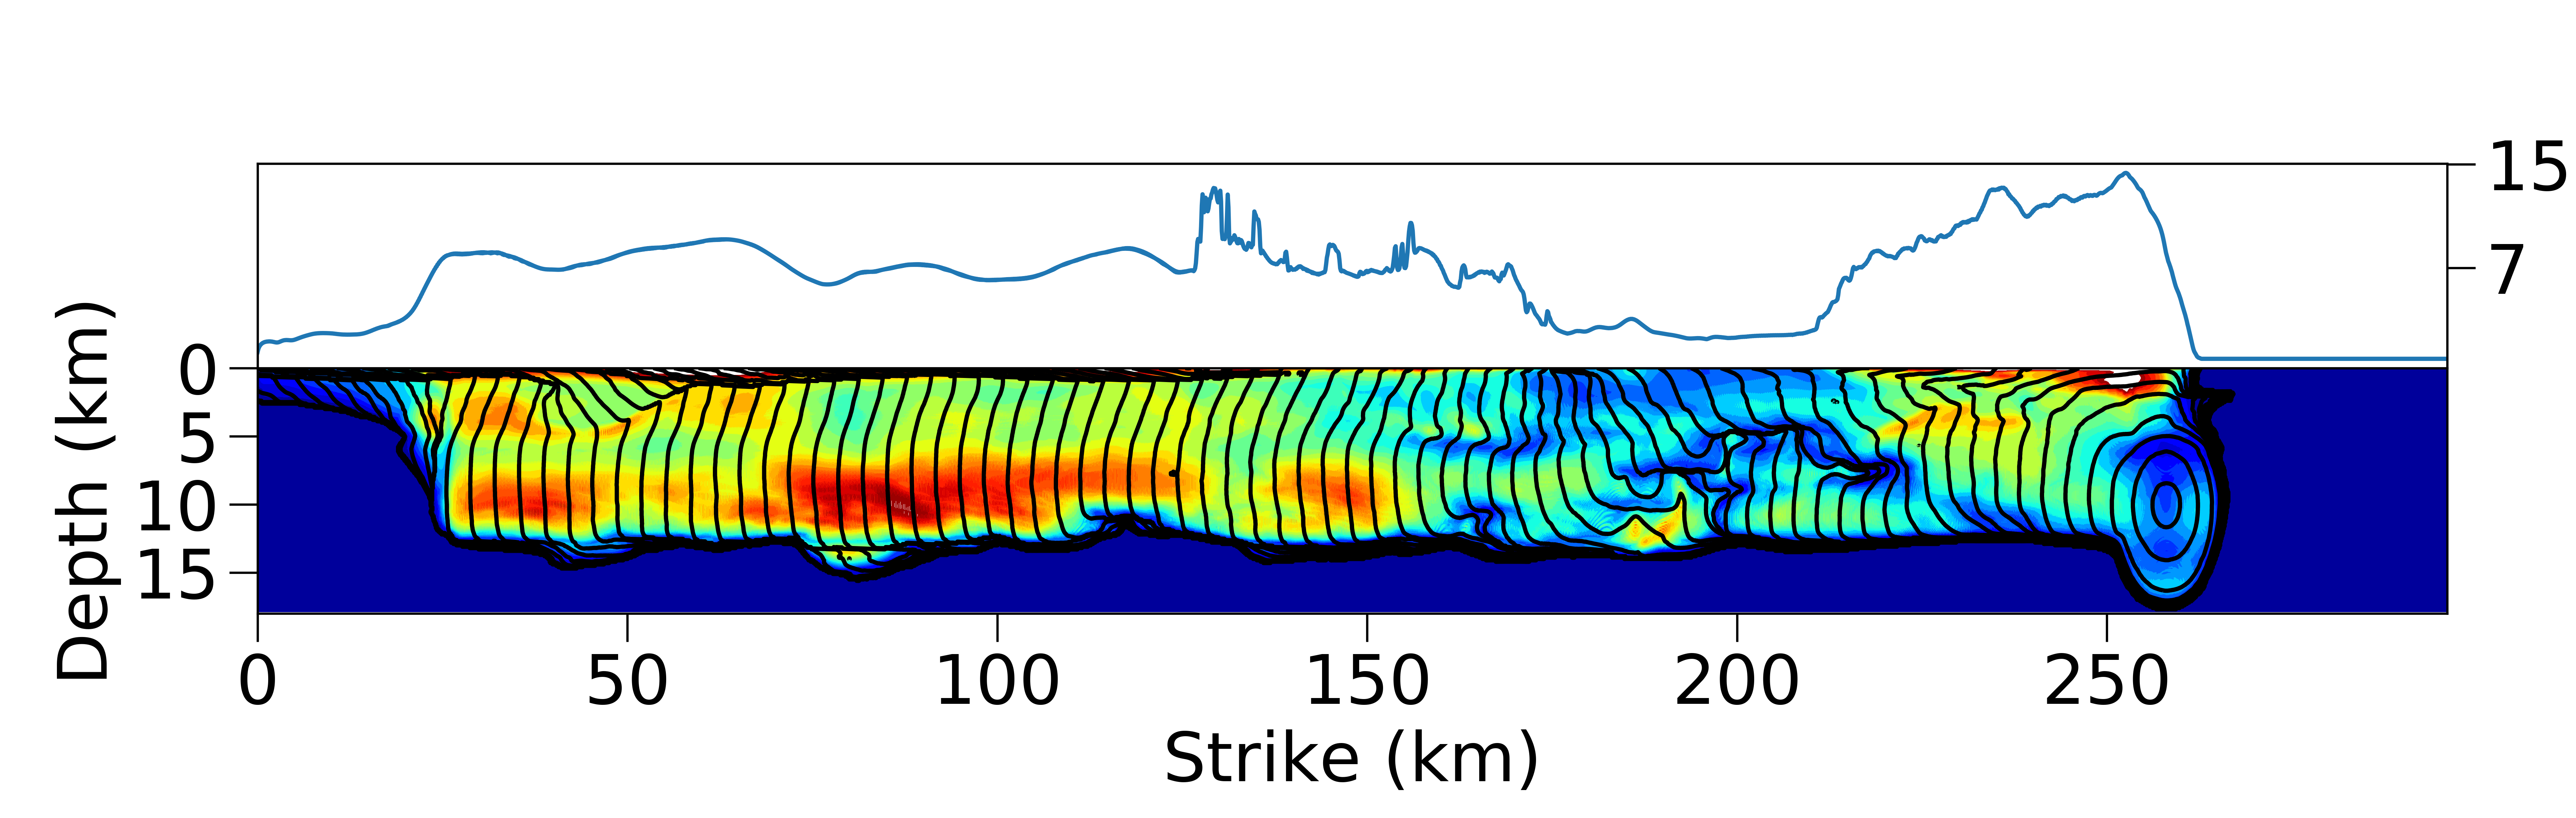
\includegraphics[width=0.9\textwidth]{figures/figure_eks_1a.png}\label{fig:eks-1a}} \\[\baselineskip]%
    \sidesubfloat[]{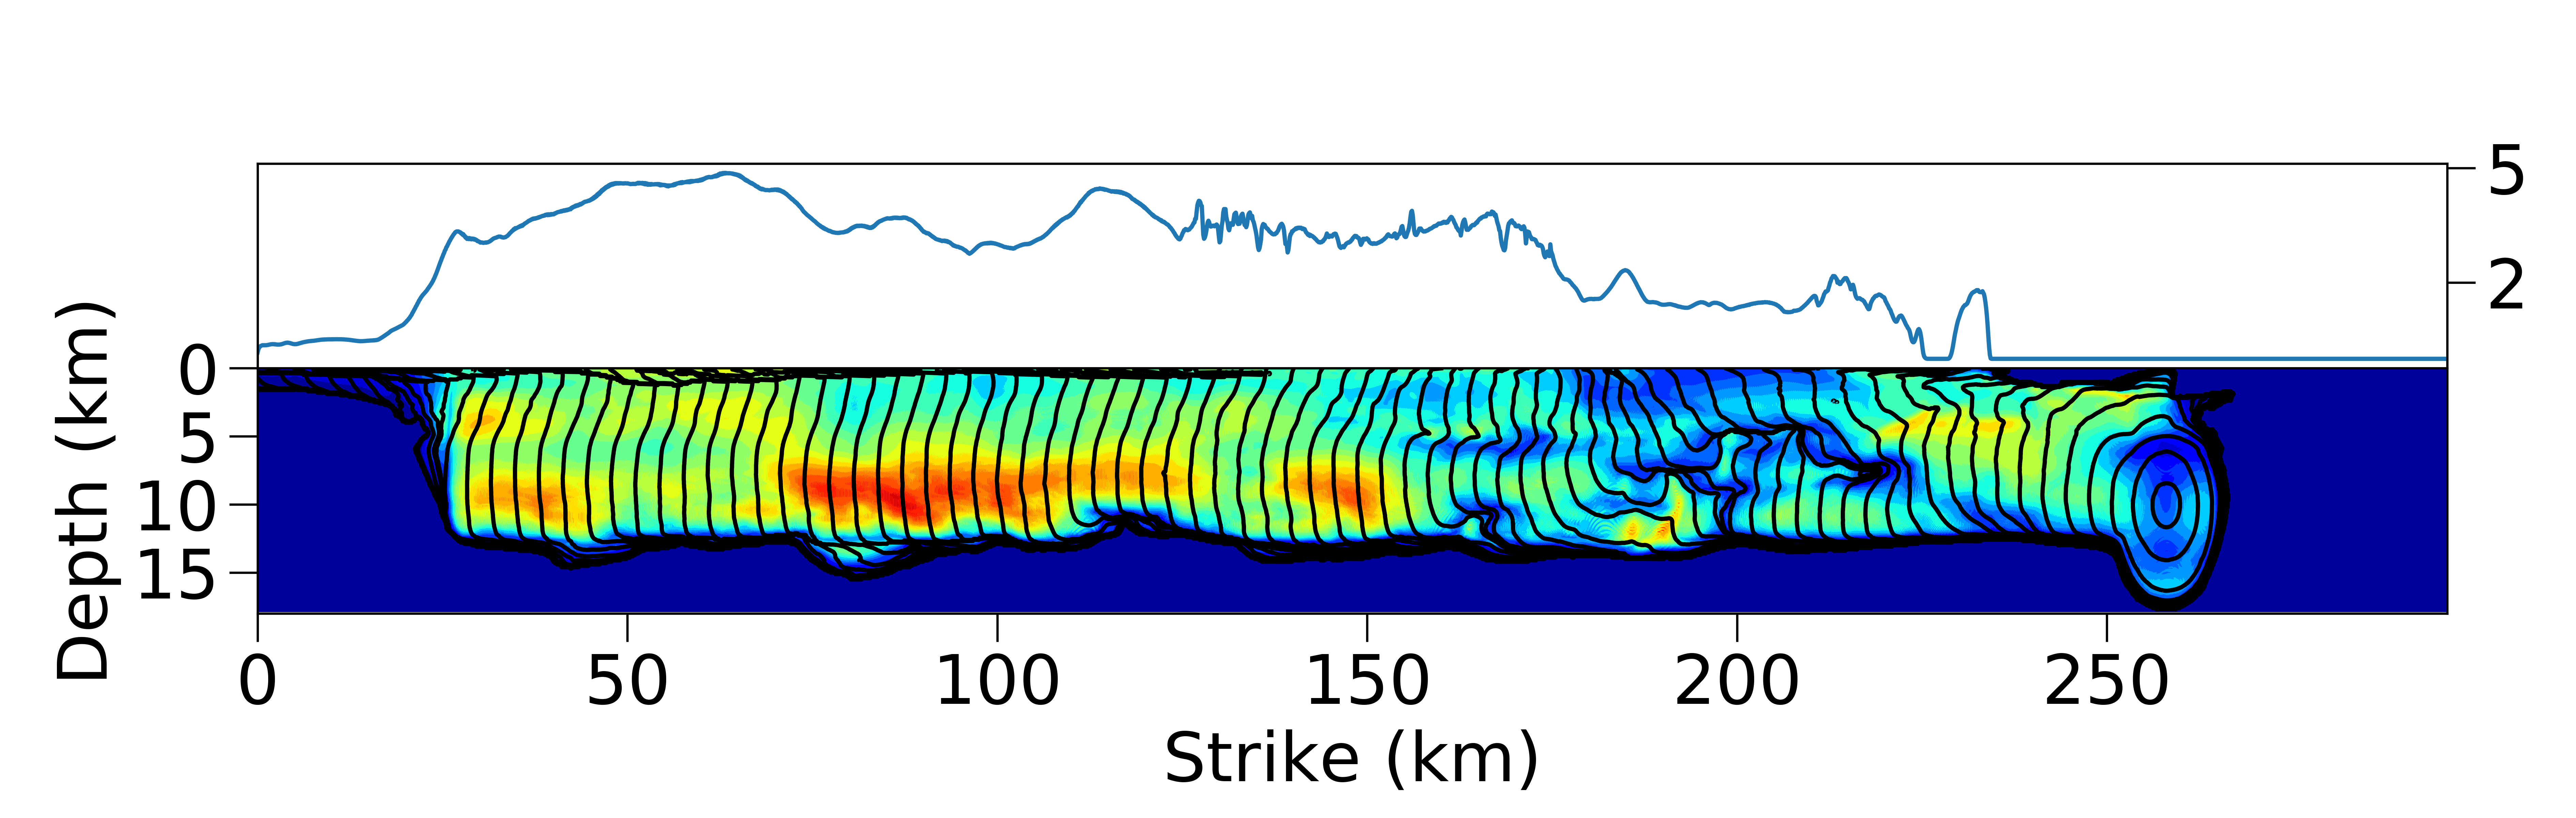
\includegraphics[width=0.9\textwidth]{figures/figure_eks_1b.png}\label{fig:eks-1b}} \\[\baselineskip]%
    \sidesubfloat[]{\includegraphics[width=0.9\textwidth]{figures/figure_eks_1c.png}\label{fig:eks-1c}} \\[\baselineskip]%
    \vspace{-3mm}
    \centering
    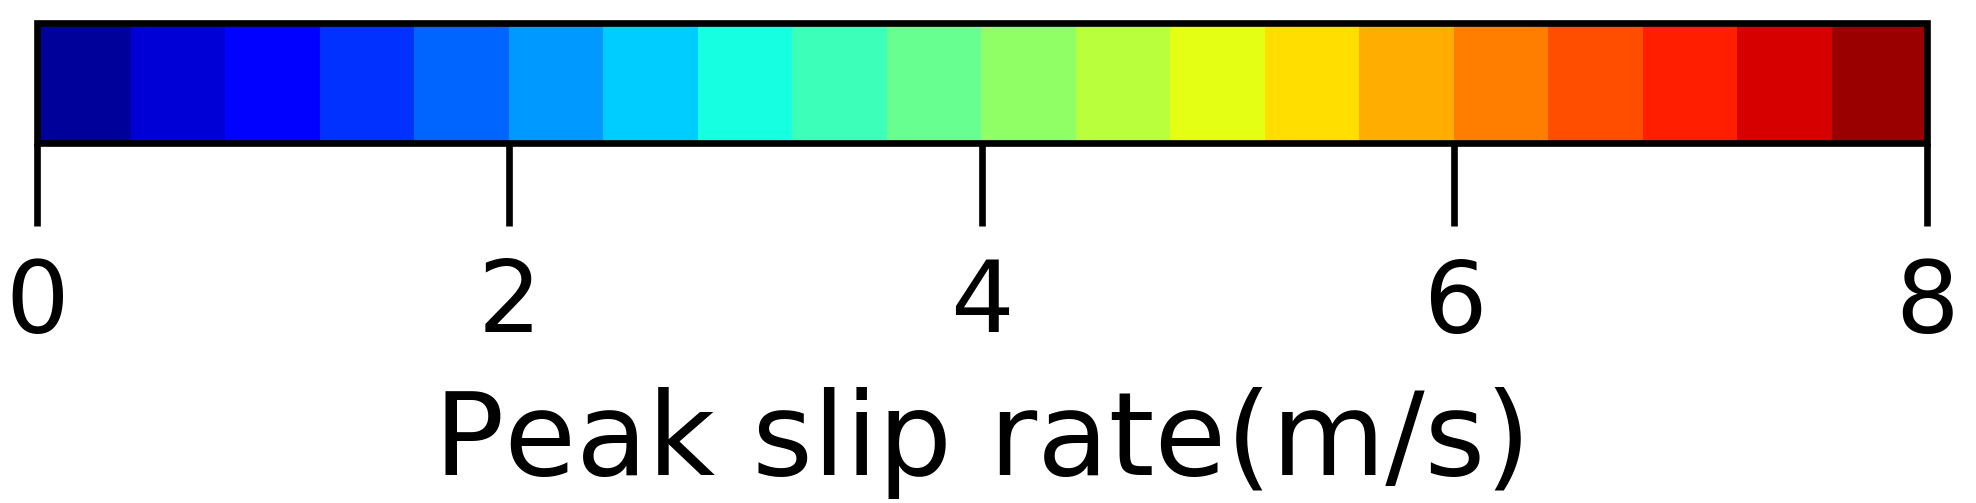
\includegraphics[width=0.3\textwidth]{figures/figure_eks_1d.png}\label{fig:eks-1d}
    \caption{Peak slip rate (PSR) simulated on the fault for ShakeOut scenario, with the surface PSR (in m/s) shown in the panel above each subplot. (a) linear, (b) sandstone (nonlinear), and (c) shale (nonlinear) results. Black contours indicate rupture time in 1 s intervals.}
    \label{fig:eks-1}
\end{figure}
\clearpage

\clearpage
\begin{figure}[!ht]
    \includegraphics[width=0.28\textwidth]{figures/figure_eks_2a.pdf}\label{fig:eks-2a} \hspace{0.02\textwidth}%
    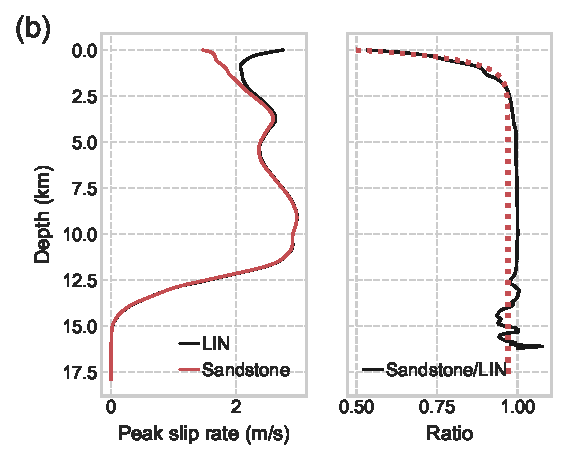
\includegraphics[width=0.28\textwidth]{figures/figure_eks_2b.pdf}\label{fig:eks-2b} \hspace{0.02\textwidth}%\hfil
    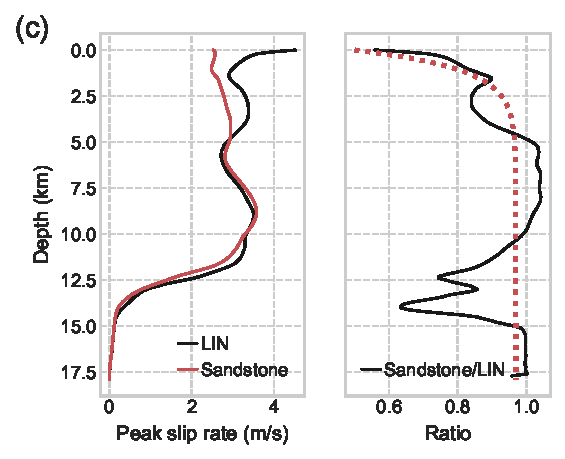
\includegraphics[width=0.28\textwidth]{figures/figure_eks_2c.pdf}\label{fig:eks-2c} % \\[\baselineskip]%
    \caption{Peak slip rate (PSR) averaged along strike against depth (left panel of each subplot) for sandstone (nonlinear) and linear models and their ratio (right panel of each subplot). (a)-(c) depit three realizations for the sandstone models with stress drop of 7, 8, and 10 MPa, respectively. Dashed red lines indicate the curves fitting the nonlinear to linear PSR ratios using \cref{eq:eks-2}.}
    \label{fig:eks-2}
\end{figure}
\clearpage


\clearpage
\begin{figure}[!ht]
    \sidesubfloat[]{\includegraphics[width=0.26\textwidth]{figures/figure_eks_3a.pdf}\label{fig:eks-3a}} \hfil
    \sidesubfloat[]{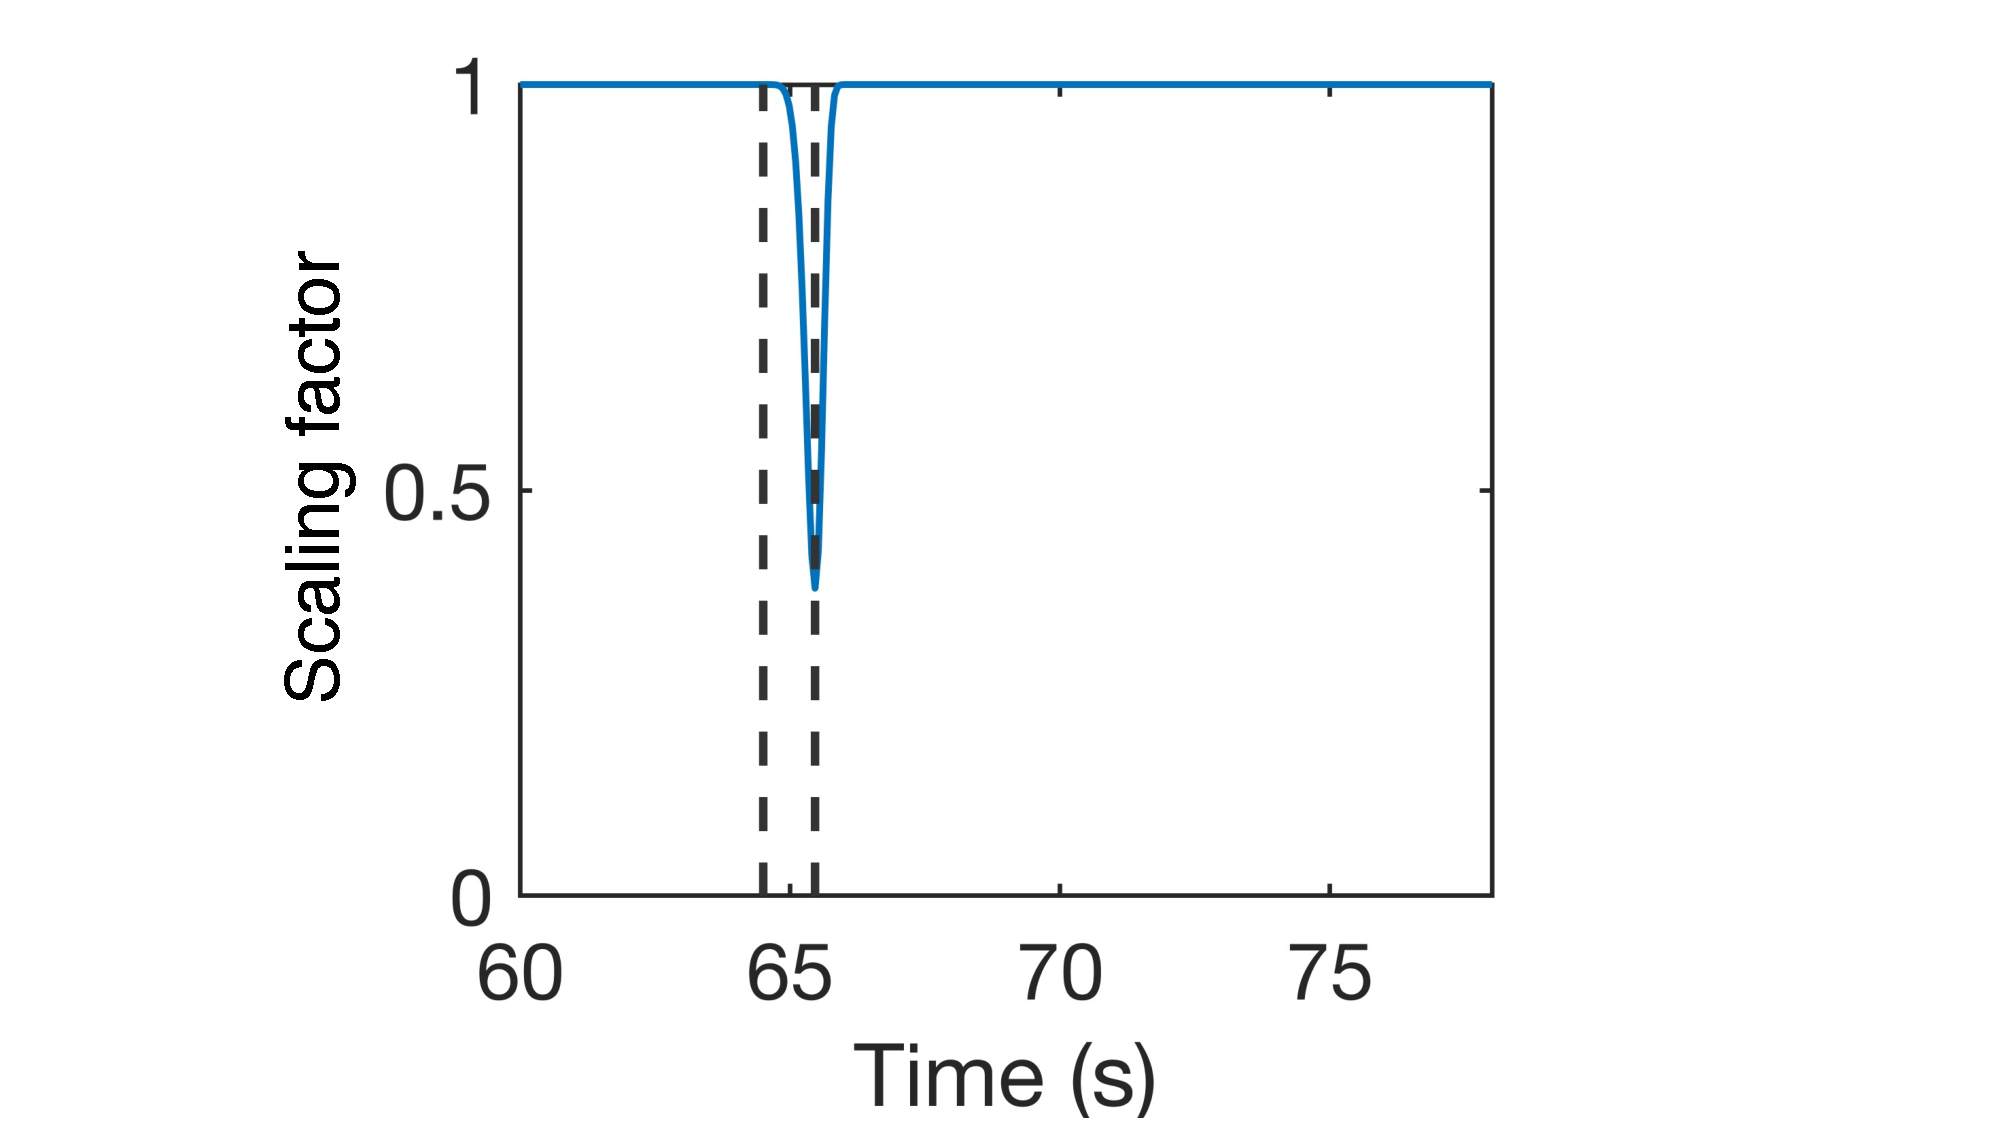
\includegraphics[width=0.26\textwidth]{figures/figure_eks_3b.pdf}\label{fig:eks-3b}} \hfil
    \sidesubfloat[]{\includegraphics[width=0.26\textwidth]{figures/figure_eks_3c.pdf}\label{fig:eks-3c}}
    \caption{(a) STF on a representative subfault (depth=0) for the linear model. (b) Time-domain scaling factors from the scaling function computed with \cref{eq:eks-2}. (c) STFs for the nonlinear model and EKS model. The black dashed lines in (a) and (b) indicate the peak time of the STF and shape functions.}
    \label{fig:eks-3}
\end{figure}
\clearpage

\clearpage
\begin{figure}[!ht]
    \includegraphics[width=0.9\textwidth]{figures/figure_eks_4.png}
    \caption{PGV distribution for the southern San Andreas fault region, obtained for (a) linear, (b) sandstone and (c) EKS model. The red rectangle depicts the LA basin region for further ground motion comparisons in \Cref{fig:eks-10}.}
    \label{fig:eks-4}
\end{figure}


\clearpage
\floatsetup[figure]{style=plain,subcapbesideposition=top,font=Large,footfont=Large}
\begin{figure}[!ht]
    \sidesubfloat[]{\includegraphics[width=0.4\textwidth]{figures/figure_eks_5a.png}\label{fig:eks-5a}} \hfil%\\[\baselineskip]%
    \sidesubfloat[]{\includegraphics[width=0.4\textwidth]{figures/figure_eks_5b.png}\label{fig:eks-5b}} \\[\baselineskip]%
    \sidesubfloat[]{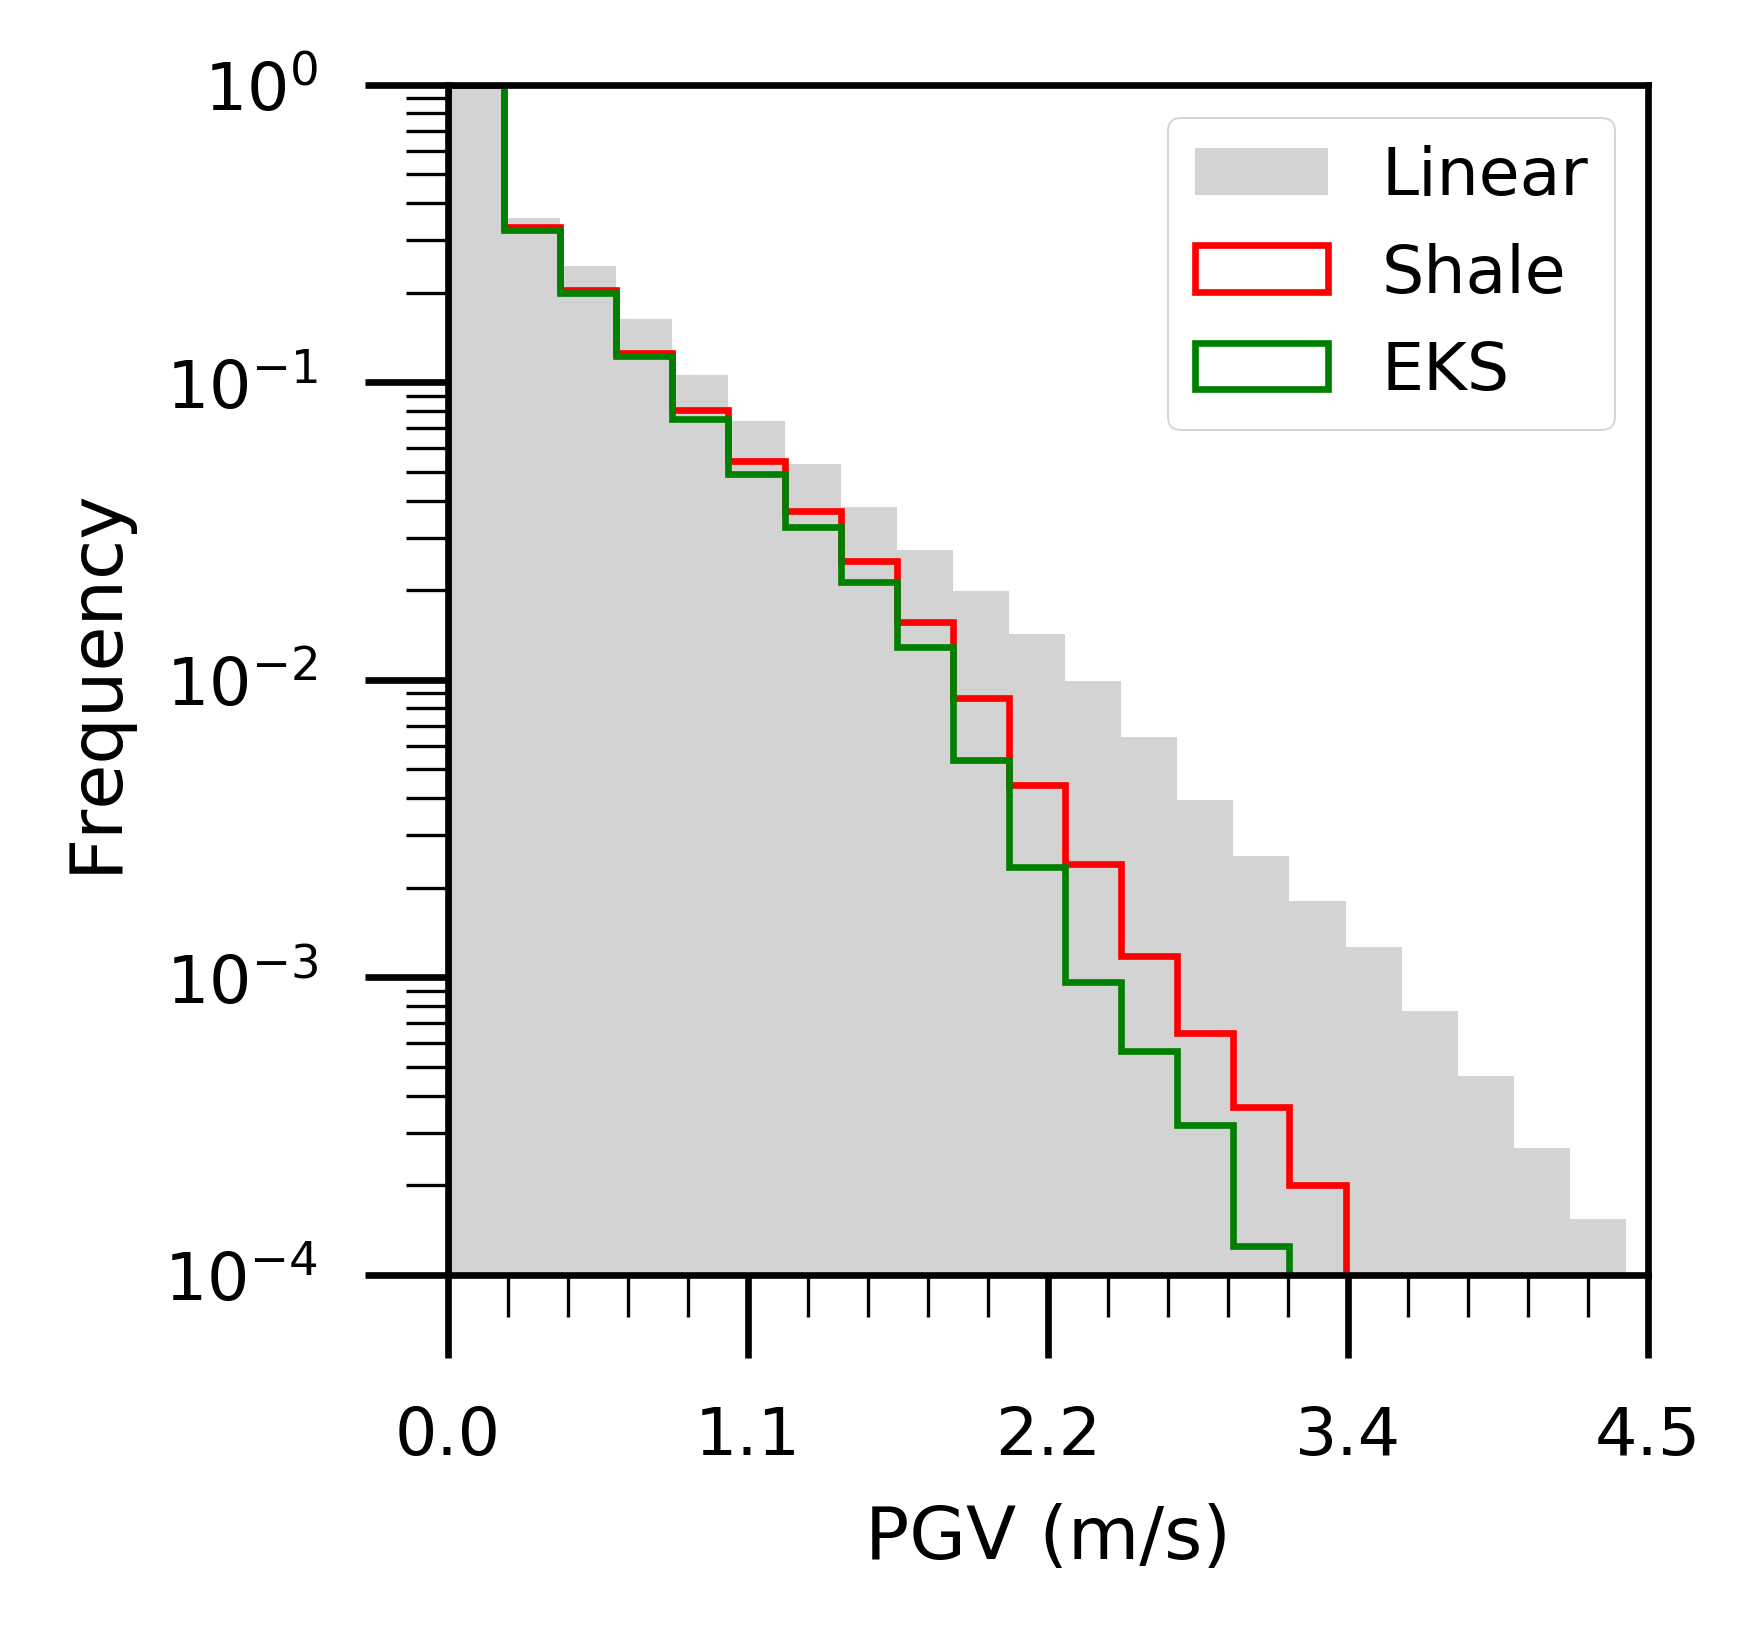
\includegraphics[width=0.4\textwidth]{figures/figure_eks_5c.png}\label{fig:eks-5c}} \hfil%\\[\baselineskip]%
    \sidesubfloat[]{\includegraphics[width=0.4\textwidth]{figures/figure_eks_5d.png}\label{fig:eks-5d}} \\[\baselineskip]

    \caption{Cumulative distribution of PGVs for linear models with stress drop of 7 (a and c) and 10 (b and d) MPa, as well as nonlinear models and the corresponding EKS models. The top row (a and b) depicts models with sandstone and the bottom row (c and d) shows models with shale.}
    \label{fig:eks-5}
\end{figure}

\clearpage
\floatsetup[figure]{style=plain,subcapbesideposition=top,font=Large,footfont=Large}
\begin{figure}[!ht]
    \sidesubfloat[]{\includegraphics[width=0.4\textwidth]{figures/figure_eks_6a.pdf}\label{fig:eks-6a}} \hfil%\\[\baselineskip]%
    \sidesubfloat[]{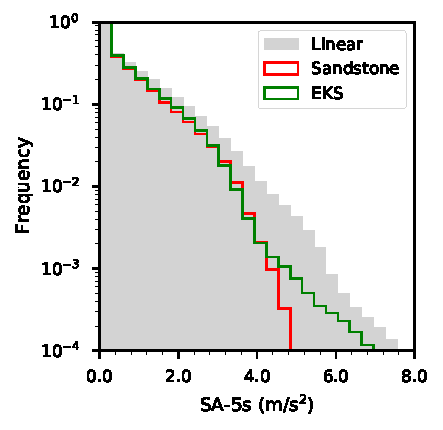
\includegraphics[width=0.4\textwidth]{figures/figure_eks_6b.pdf}\label{fig:eks-6b}} \\[\baselineskip]%
    \sidesubfloat[]{\includegraphics[width=0.4\textwidth]{figures/figure_eks_6c.pdf}\label{fig:eks-6c}} \hfil%\\[\baselineskip]%
    \sidesubfloat[]{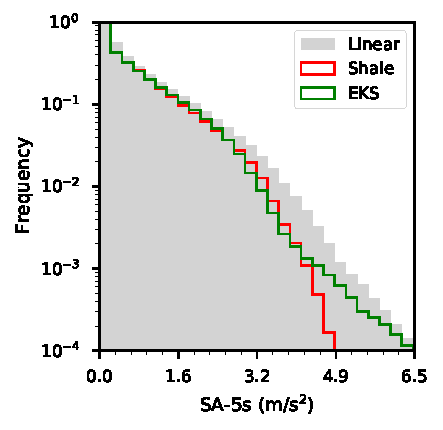
\includegraphics[width=0.4\textwidth]{figures/figure_eks_6d.pdf}\label{fig:eks-6d}}

    \caption{Same as \Cref{fig:eks-5}, but for SA-5s comparisons.}
    \label{fig:eks-6}
\end{figure}

\clearpage
\floatsetup[figure]{style=plain,subcapbesideposition=top,font=Large,footfont=Large}
\begin{figure}[!ht]
    \sidesubfloat[]{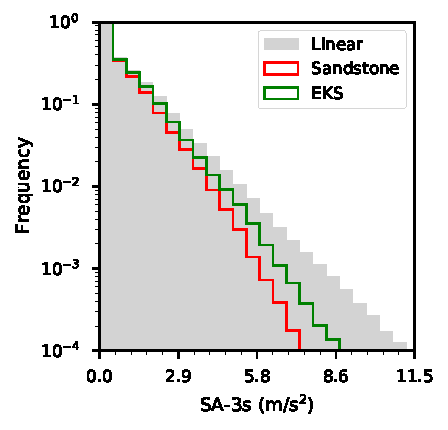
\includegraphics[width=0.4\textwidth]{figures/figure_eks_7a.pdf}\label{fig:eks-7a}} \hfil%\\[\baselineskip]%
    \sidesubfloat[]{\includegraphics[width=0.4\textwidth]{figures/figure_eks_7b.pdf}\label{fig:eks-7b}} \\[\baselineskip]%
    \sidesubfloat[]{\includegraphics[width=0.4\textwidth]{figures/figure_eks_7c.pdf}\label{fig:eks-7c}} \hfil%\\[\baselineskip]%
    \sidesubfloat[]{\includegraphics[width=0.4\textwidth]{figures/figure_eks_7d.pdf}\label{fig:eks-7d}}

    \caption{Same as \Cref{fig:eks-5}, but for SA-3s comparisons.}
    \label{fig:eks-7}
\end{figure}

\clearpage
\floatsetup[figure]{style=plain,subcapbesideposition=top,font=Large,footfont=Large}
\begin{figure}[!ht]
    \sidesubfloat[]{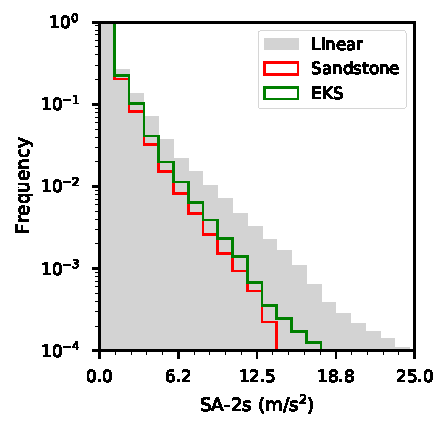
\includegraphics[width=0.4\textwidth]{figures/figure_eks_8a.pdf}\label{fig:eks-8a}} \hfil%\\[\baselineskip]%
    \sidesubfloat[]{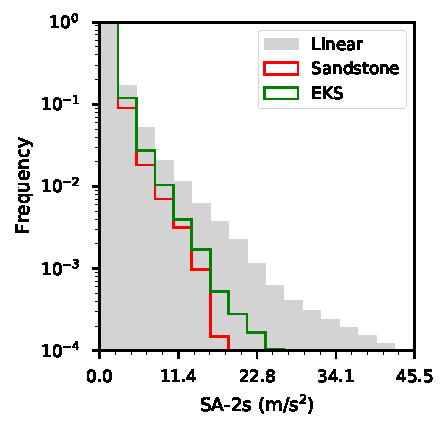
\includegraphics[width=0.4\textwidth]{figures/figure_eks_8b.pdf}\label{fig:eks-8b}} \\[\baselineskip]%
    \sidesubfloat[]{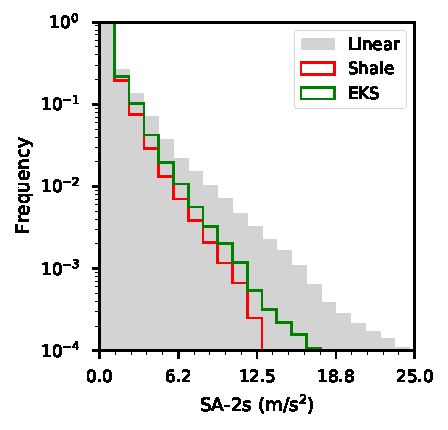
\includegraphics[width=0.4\textwidth]{figures/figure_eks_8c.pdf}\label{fig:eks-8c}} \hfil%\\[\baselineskip]%
    \sidesubfloat[]{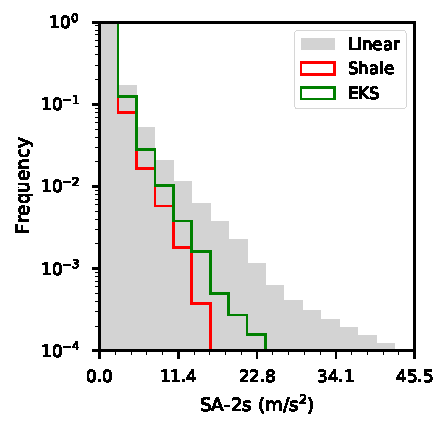
\includegraphics[width=0.4\textwidth]{figures/figure_eks_8d.pdf}\label{fig:eks-8d}}

    \caption{Same as \Cref{fig:eks-5}, but for SA-2s comparisons.}
    \label{fig:eks-8}
\end{figure}

\clearpage
\floatsetup[figure]{style=plain,subcapbesideposition=top,font=Large,footfont=Large}
\begin{figure}[!ht]
    \sidesubfloat[]{\includegraphics[width=0.4\textwidth]{figures/figure_eks_9a.pdf}\label{fig:eks-9a}} \hfil%\\[\baselineskip]%
    \sidesubfloat[]{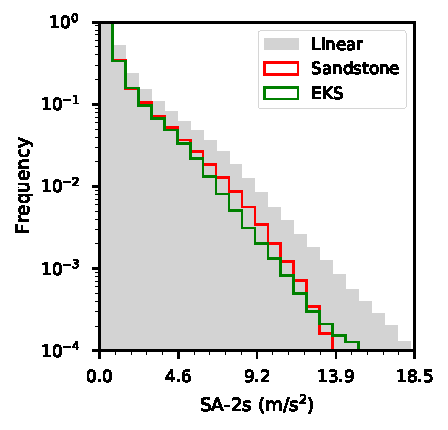
\includegraphics[width=0.4\textwidth]{figures/figure_eks_9b.pdf}\label{fig:eks-9b}} \\[\baselineskip]%
    \sidesubfloat[]{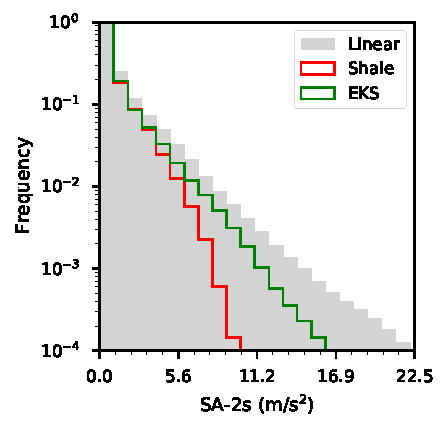
\includegraphics[width=0.4\textwidth]{figures/figure_eks_9c.pdf}\label{fig:eks-9c}} \hfil%\\[\baselineskip]%
    \sidesubfloat[]{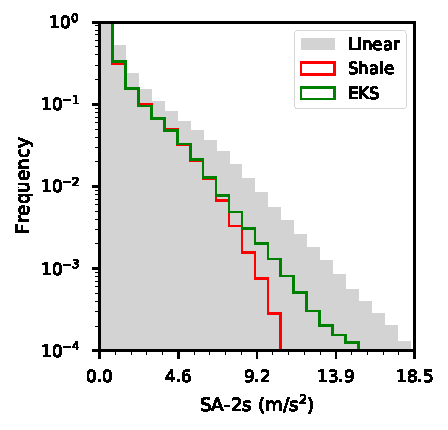
\includegraphics[width=0.4\textwidth]{figures/figure_eks_9d.pdf}\label{fig:eks-9d}}

    \caption{Same as \Cref{fig:eks-8}, but the rupture direction is reversed to NW-SE for all models.}
    \label{fig:eks-9}
\end{figure}


\clearpage
\floatsetup[figure]{style=plain,subcapbesideposition=top,font=Large,footfont=Large}
\begin{figure}[!ht]
    \sidesubfloat[]{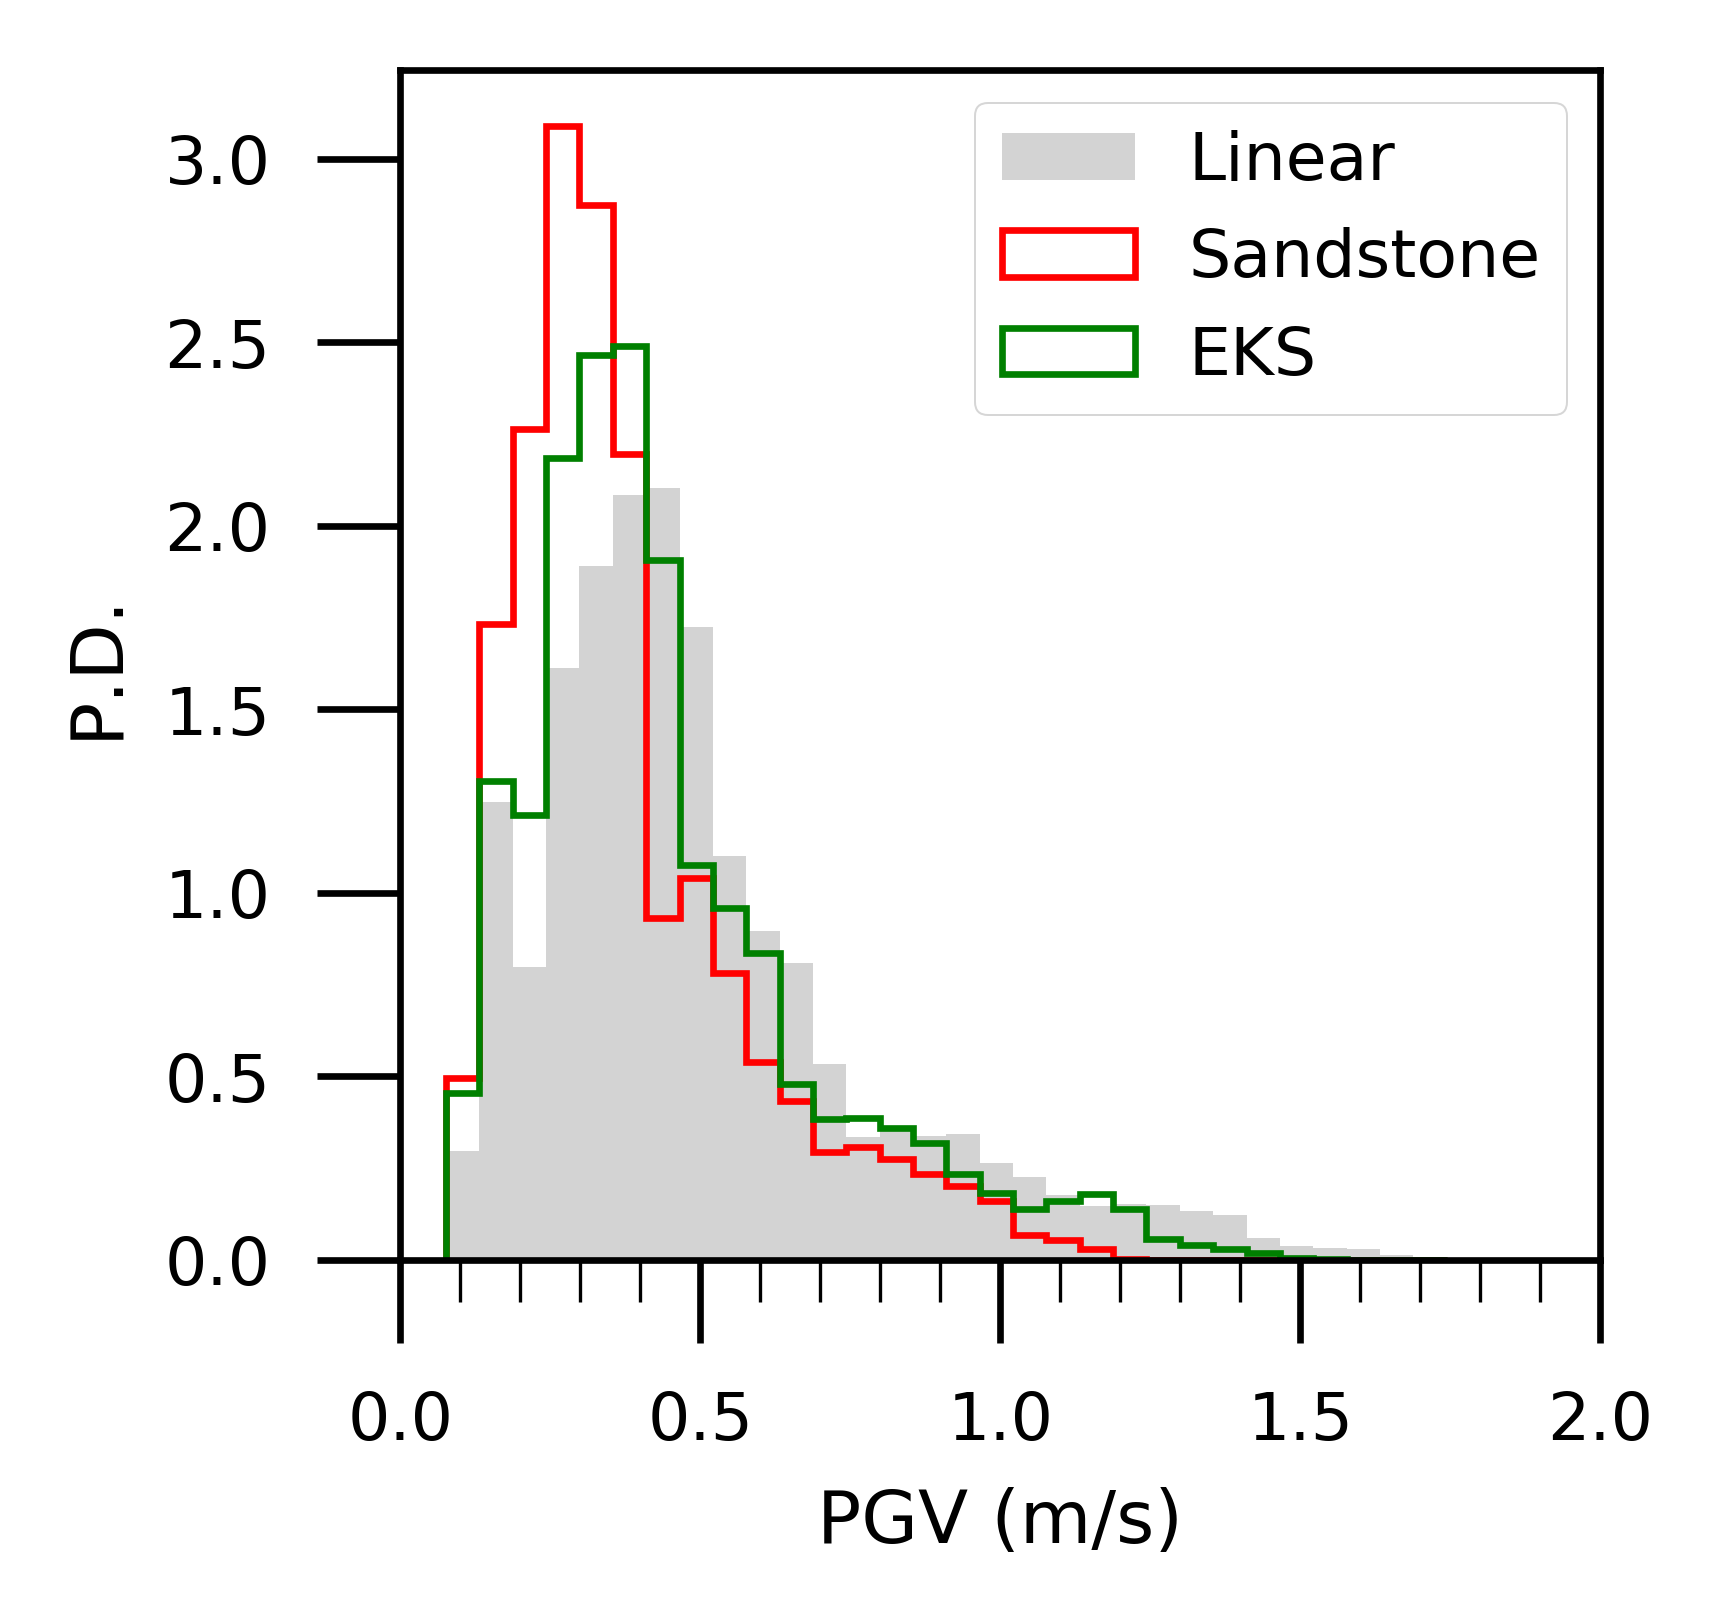
\includegraphics[width=0.4\textwidth]{figures/figure_eks_10a.png}\label{fig:eks-10a}} \hfil%\\[\baselineskip]%
    \sidesubfloat[]{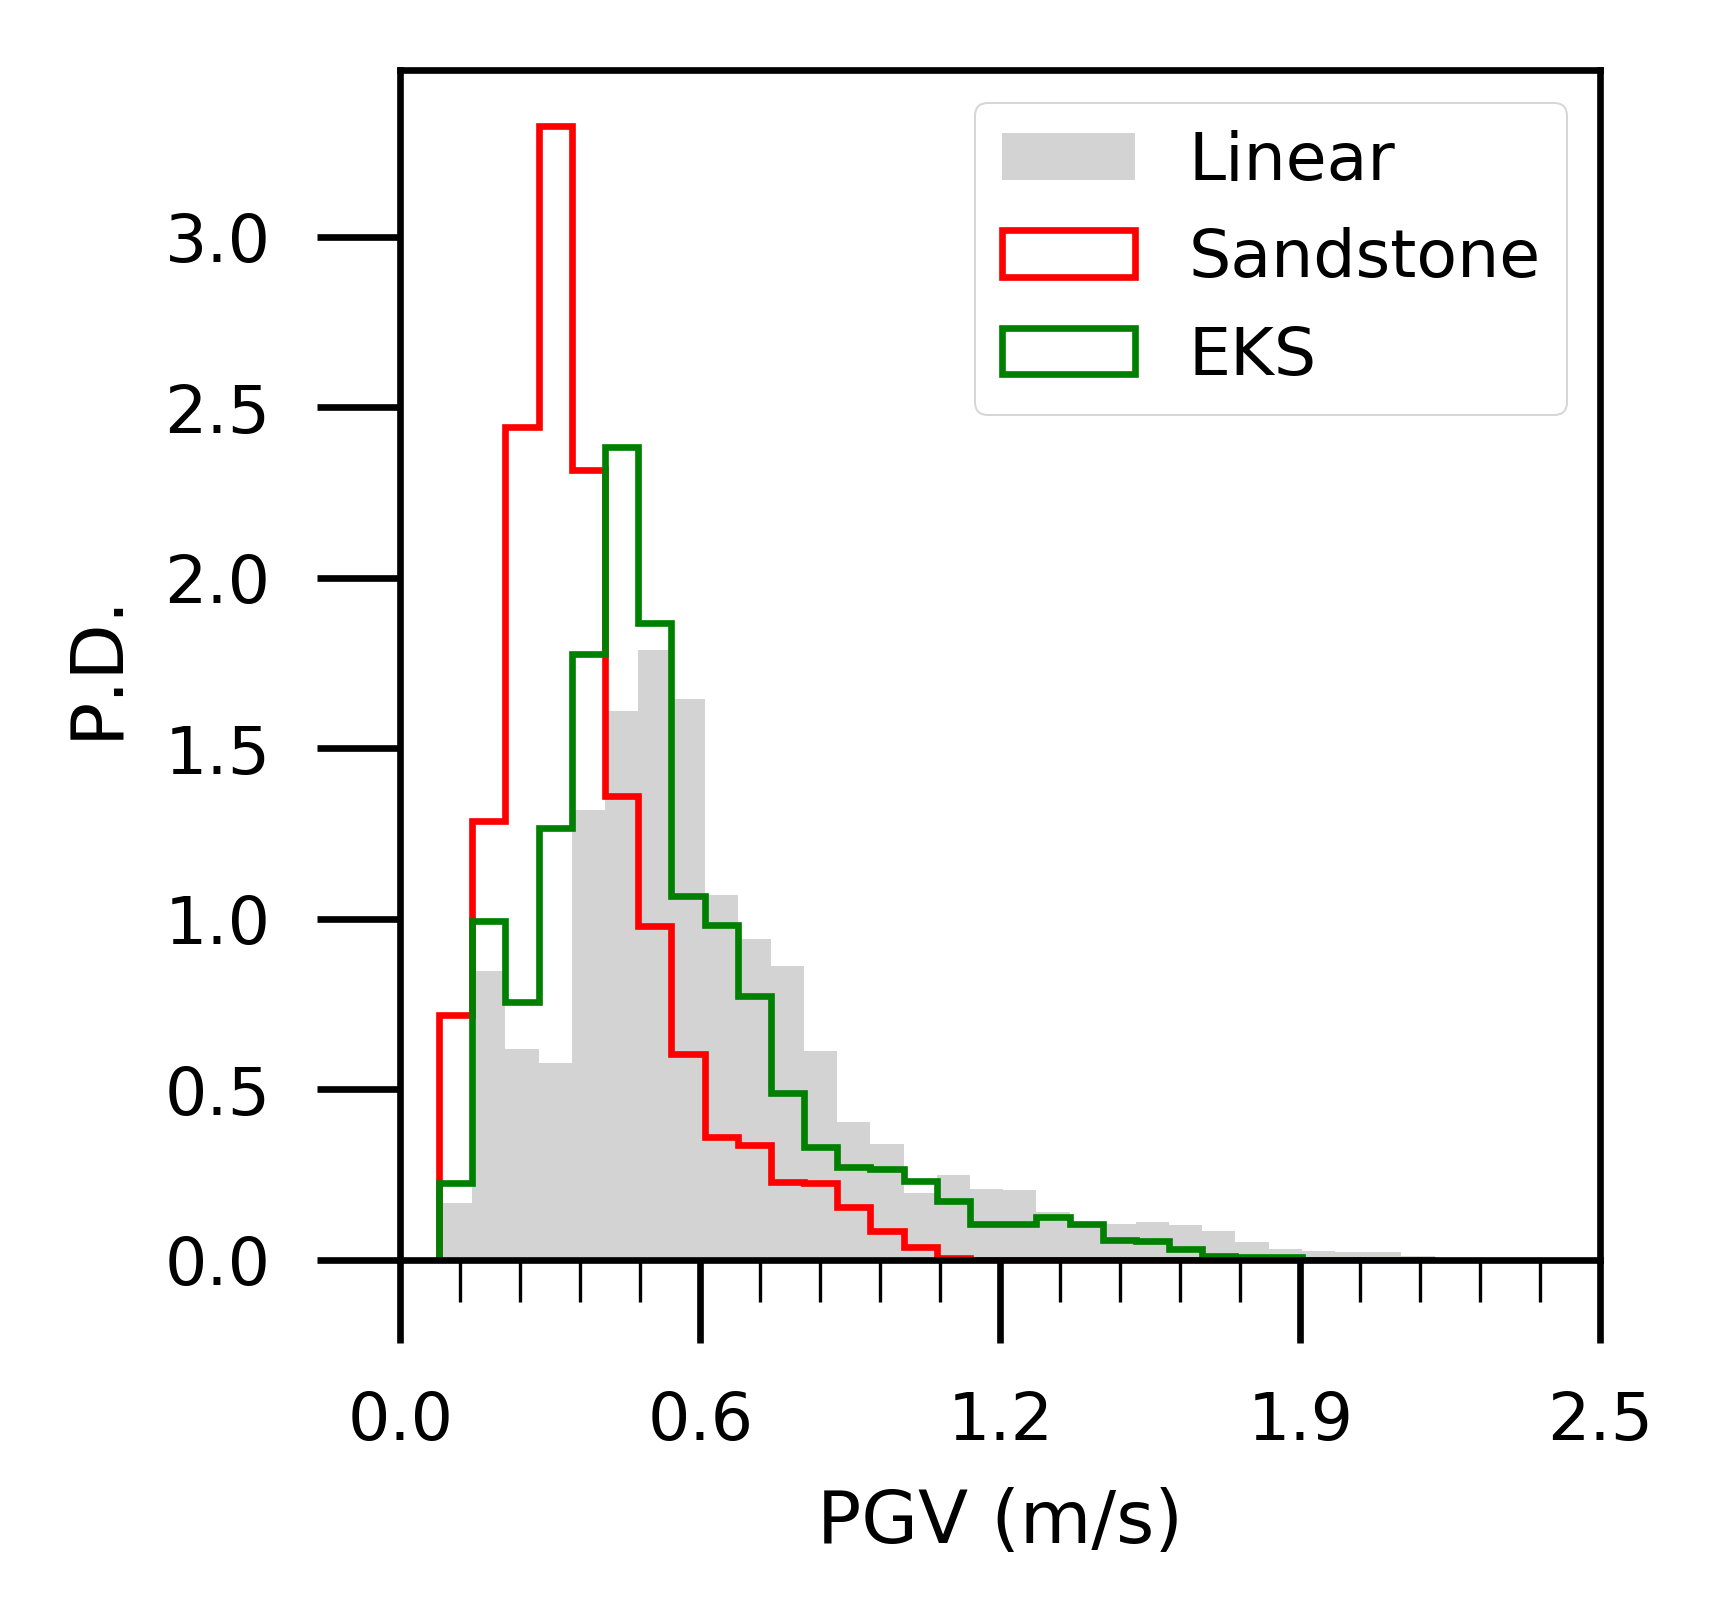
\includegraphics[width=0.4\textwidth]{figures/figure_eks_10b.png}\label{fig:eks-10b}} \\[\baselineskip]%
    \sidesubfloat[]{\includegraphics[width=0.4\textwidth]{figures/figure_eks_10c.png}\label{fig:eks-10c}} \hfil%\\[\baselineskip]%
    \sidesubfloat[]{\includegraphics[width=0.4\textwidth]{figures/figure_eks_10d.png}\label{fig:eks-10d}}

    \caption{Probability density (P.D.) histograms of PGVs in the Los Angeles Basin area.}
    \label{fig:eks-10}
\end{figure}

\clearpage

%% supplement
% \setcounter{table}{0}
% \setcounter{figure}{0}
% \numberwithin{figure}{chapter}
% \numberwithin{table}{chapter}
% \renewcommand{\thetable}{S\arabic{chapter}.\arabic{table}}
% \renewcommand{\thefigure}{S\arabic{chapter}.\arabic{figure}}
% \newpage
% \section*{Supplementary Materials}
% \addcontentsline{toc}{section}{\protect\numberline{}Supplementary Materials}

% This supplement includes.




\renewcommand{\thetable}{\arabic{table}}
\renewcommand{\thefigure}{\arabic{figure}}

\numberwithin{figure}{chapter}
\numberwithin{table}{chapter}

%\endrefsection